\begin{wrapfigure}{L}{0.5\textwidth}
    \begin{center}
        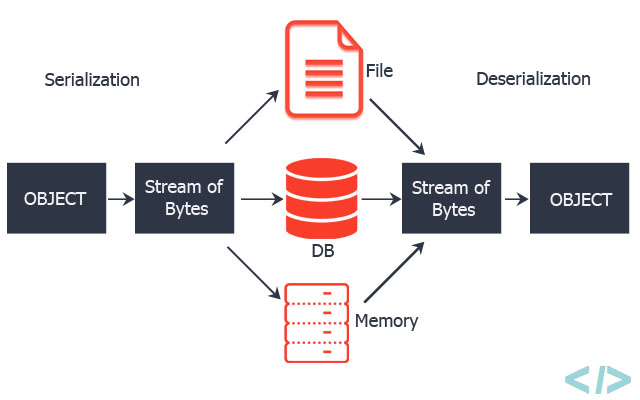
\includegraphics[width=0.5\textwidth]{header-picture}
    \end{center}
    \caption*{pc: \href{https://www.codenuclear.com/serialization-deserialization-java/}{codenuclear.com}}
\end{wrapfigure}

Serialization (also known as marshalling) is a technique used to share the state of data in memory.  

During serialization, data structures and objects are converted into a stream of bytes, which then can be stored on a disk or shared over a network. Serialization becomes useful when data must be reconstructed via deserialization (or unmarshalling): the serialized stream is used to recreate the original object in memory, and the new object is semantically equivalent to when it was serialized. 

In this lab we will explore a brief history of various serialization techniques and understand how computer files work. Then we will investigate how we can implement these techniques into microcontroller driven systems. In the following labs, we will actually implement two examples of serialization in ArduinoC and corresponding deserialization. 

\subsection{What's the point?}
We mentioned that serialization is used to share the state of data in memory—but what does this really mean? When would you use it?

In a computer program, an object's lifespan is relatively short. The object may be removed by a garbage collector when it is no longer needed, and will most certaintly be destroyed when the program terminates. 

Sometimes, we would like to "save" this object—or at least everything about it—and be able to "revive" it at a later time (perhaps even on another program and computer). An example of when we'd like to do this is communicating efficiently between different microcontrollers, or saving program data to an SD card to analyze it more effectively later on.

Serialization will help us accomplish these goals!
